%!TEX root = ../main.tex
%%%%%%%%%%%%%%%%%%%%%%%%%%%%%%%%%%
% Links:
%
% Difficulty: Companies: 
%%%%%%%%%%%%%%%%%%%%%%%%%%%%%%%%%%


%\begin{figure} \centering
%   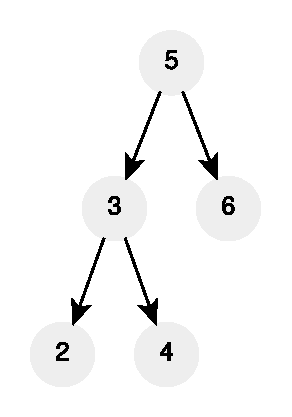
\includegraphics[width=\textwidth]{sources/remove_all_occurrences_unsorted_array_inplace/images/example1}
%   \caption[Sample short cpation]{Sample Caption}.
%   \label{fig:remove_all_occurrences_unsorted_array_inplace:example1} \end{figure}

\chapter{Remove all occurrences -  unsorted array}
\label{ch:remove_all_occurrences_unsorted_array_inplace}
\section*{Introduction}
The problem covered in this chapter asks us to implement a common operations: removeing all
elements satisfying specific criterium from a collection. This problem has many similarities to
the one discussed in Chapter \ref{ch:remove_duplicated_sorted_array_inplace} and as a consequence
they share the same general approach to their solution. 

There are many variations of this problem but the most common being  where the
collection is a simple array or a vector of integers and we are asked to remove all the elements
equal to a given integer. On this ocassion, however,  we will discuss a more generalized version where the 
collection is of a generic type \inline{T} and the criterium is given in the form of a unary
function returning a boolean\footnote{This type of function is commonly known as
\textit{predicates}.}. 

If you are asked to solve this particular problem version during an interview, you should be able to easily specialise what is discussed here in the moment.

\section{Problem statement}
\begin{exercise}
\label{example:remove_all_occurrences_unsorted_array_inplace:exercice1}
Write a function that -  given a collection $I$ of elements of type \inline{T}
 and a predicate function
 $p$ with signature \inline{bool(const T&)} -  rearranges $I$ in such a way that all the $0 \leq k
 \leq |I|$ elements satisfying $p$ in $I$ are moved to the front. The function should returns $k$.

 Moreover, the relative order of the elements  satisfying $p$ should be preserved. If both elements
 at indices $n$ and $m$ satisfy the predicate $p$  and $I_n$ comes before $I_m$ then when the
 function returns, their relative order is unchanged albeit they both might be moved to new
 locations.
 
	%example1
	\begin{example}
		\label{example:remove_all_occurrences_unsorted_array_inplace:example1}
		\hfill \\
		Given $I = \{{4, 1, 1, 2, 1, 3\}}$ and a function $p$ returning true if its input argument is an even number, false otherwise, the function returns $4$. The first $4$ elements of $I$ are $\{1,1,1,3\}$. 
		
	\end{example}

	\begin{example}
		\label{example:remove_all_occurrences_unsorted_array_inplace:example2}
		\hfill \\
		Given $I = \{4, 1, 1, 2, 1, 3\}$ and a function $p$ returning true if its input argument is odd, the function returns $2$. At this point, the first $2$ elements of $I$ are $\{4,2\}$. 
		
	\end{example}
\end{exercise}

\section{Clarification Questions}

\begin{QandA}
	\item \begin{questionitem} \begin{question} What should the content be of $I$ from index $k+1$ and after?  \end{question} 	 
    \begin{answered}
		\textit{There are no constraints on the content of those cells of $I$.}
	\end{answered} \end{questionitem}
	
\end{QandA}

\section{Discussion}
\label{remove_all_occurrences_unsorted_array_inplace:sec:discussion}
This problem could be restated as: \textit{Implement the
\inline{remove_if}\footnote{\url{https://en.cppreference.com/w/cpp/algorithm/remove}}} function from
the C++ STL. So it would not be surprising if, during an interview,  it could come-up as a
one-liner as  shown in Listing \ref{list:remove_all_occurrences_unsorted_array_inplace:STL}
\footnote{Notice the similarities with Listing \ref{list:remove_duplicated_sorted_array_inplace_stl} for the problem in Chapter \ref{ch:remove_duplicated_sorted_array_inplace}}.

\lstinputlisting[language=c++, caption={One-liner solution using the STL functions \inline{distance} and \inline{remove_if}},label=list:remove_all_occurrences_unsorted_array_inplace:STL]{sources/remove_all_occurrences_unsorted_array_inplace/remove_all_occurrences_unsorted_array_inplace_solution1.cpp}


This algorithm has a linear time and constant space complexity, which is pretty much as good as it gets considering you must at least read all the elements in the input array. 
It is worth mentioning, however, that  if you present this solution to an interviewer you can expect to be asked to implement the logic behind \inline{std::remove_if}
 itself as this is the core of the problem. 

\subsection{Linear time and linear space solution}
\label{remove_all_occurrences_unsorted_array_inplace:sec:bruteforce}
There is a straightforward way of solving this problem that has the added benefit of occupying
only a couple of lines and of being very clear and simple. The idea is that we can use an additional
linear amount of space to temporarily store the valid (dissatisfying the predicate \inline{p}
) elements, and in a subsequent
phase move them to the front of \inline{I}
. Listing \ref{list:remove_all_occurrences_unsorted_array_inplace:copy} shows a possible implementation of this idea.

\lstinputlisting[language=c++, caption={Linear space solution using the \inline{std::copy} family of functions from the STL.},label=list:remove_all_occurrences_unsorted_array_inplace:copy]{sources/remove_all_occurrences_unsorted_array_inplace/remove_all_occurrences_unsorted_array_inplace_solution2.cpp}


This solution only works correctly for types that can be copied. As such, the interviewer could
 ask you to fix this; in which case you can loop over \inline{I}
 and \inline{temp}
 and
\href{https://en.cppreference.com/w/cpp/utility/move}{\inline{move}
}\footnote{\inline{std::move}
 is used to indicate that an object t may be "moved from", i.e. allowing the efficient transfer of resources from t to another object without the need for an explicit copy.}
 the elements around instead.



\subsection{Linear time and constant space solution}
\label{remove_all_occurrences_unsorted_array_inplace:sec:constant_space}

The idea discussed in Section \ref{remove_all_occurrences_unsorted_array_inplace:sec:bruteforce} can quite easily be modified so that we avoid using additional linear
space. We could use \inline{std::move} the elements of $I$ into $I$ itself in the same way as we did for the problem covered in Chapter \ref{ch:remove_duplicated_sorted_array_inplace}
while discussing the solution \ref{list:remove_duplicated_sorted_array_inplace}. 

Here we use exactly the same approach of two pointers $x$ and $y$:
\begin{enumerate}
	\item  $x$ keeps track of the new front to $I$. It points to the end of the portion of $I$ (starting at index $0$ and ending at $x-1$) containing all the valid elements found so far;
	\item $y$ is a pointer to the next element not yet processed in $I$.
\end{enumerate}

Listing \ref{list:remove_all_occurrences_unsorted_array_inplace:constant_space} implements this idea.

\lstinputlisting[language=c++, caption={Constant space solution using a two pointer approach.},label=list:remove_all_occurrences_unsorted_array_inplace:constant_space]{sources/remove_all_occurrences_unsorted_array_inplace/remove_all_occurrences_unsorted_array_inplace_solution3.cpp}



At the beginning of the execution the algorithm moves $x$ forward. All the valid elements that are already
at the front of $I$ stay untouched as they are already in the right locations.
At this point, $x$ points either to the first invalid element in $I$ or to one element past $I$.
In the second scenario, there is no more work to do. All the elements are valid to begin with, and the second \inline{while}

will not even start. $I$ is left unchanged.
In the first scenario, we will use $y$ to scan the remaining elements of $I$ past $x$, and we move each valid element we encounter 
into the location pointed by $x$. When this happens $x$ is moved forward as the portion of valid elements grew by one element. 

Notice that the invariant $x \leq y$ is always respected as:
\begin{itemize}
	\item it holds before the beginning of the loop;
	\item $x$ is incremented at the same rate or less compared to $y$.
\end{itemize}

At the end of this process, we are left with $y$ pointing to the one element past $I$ and $x$ pointing to one cell after the last valid element of the newly rearranged $I$.